\section{Background and Related Work}
\label{sec:background}

This section will first describe background information on BECS
equipment and then the general state-of-the-art in differential
privacy.

\subsection{Agricultural IoT Data}
\label{sec:agIoT}

BECS Technology's equipment are fairly typical devices
in the Internet of Things (IoT).
The devices monitor various aspects of animal husbandry:
barn temperature, feed stocks, feed consumption, water consumption, etc.
In addition, our equipment interfaces with equipment from
other manufacturers for ventilation control, etc.
Based on this information, the various controllers take actions
(starting/stopping feed delivery augers, starting/stopping ventilation
fans, etc.) to maintain
the barn environment at the proper levels and ensure the animals are
properly fed.
Alarm conditions trigger notifications to service personnel.
Sensor values and actions are logged,
and these logs are frequently used when diagnosing the causes
of alarms or other anomalous events.
Remote access to all of the above information is
clearly to the benefit of the animal owners/farmers.

While the notion of IoT might be new,
the fundamental capability to access controller information remotely
is not.  BECS Technology's controllers have supported remote communications
for more than 2 decades.
Early controllers used modems attached to the telephone network
(an option still available for those that need it), today
controllers support TCP/IP connectivity via the Internet.

Remote capabilities include viewing of current status, downloading
of data logs, and configuration of the equipment.
Figure~\ref{console} shows a screenshot of the Feed-Link dashboard
for a specific farm with 3 barns (organized into 2 distinct sides, North
and South) in which the 12 grain bins have
been instrumented.
Note that, as described in Section~\ref{sec:plan}, BECS Technology's
equipment is sold, private-label, under the AP and Cumberland brands
of GSI, a global agriculture company.
The banner near the top indicates we are viewing data from the
``Smith and Jones'' farm from mid-July to mid-August.

There are links on the middle portion of the screen that drill down
into more detailed status reports, notifications of anomolies, and
options to download the logs in a spreadsheet-compatible form.
This is also where the user indicates the range of data he/she wishes
to view.

Each plot along the bottom shows bin weight over a one month timeframe
for each bin and also totals for each side of each barn.
Vertical jumps in the graphs represent feed deliveries, and the linear
downward slope shows feed consumption.  Nominally, bins are paired for
each side of the barn, with one bin operational at a time, so there
should also be portions of the plots that are horizontal, indicating
that bin is not providing feed.

\begin{figure}[t]
 \center
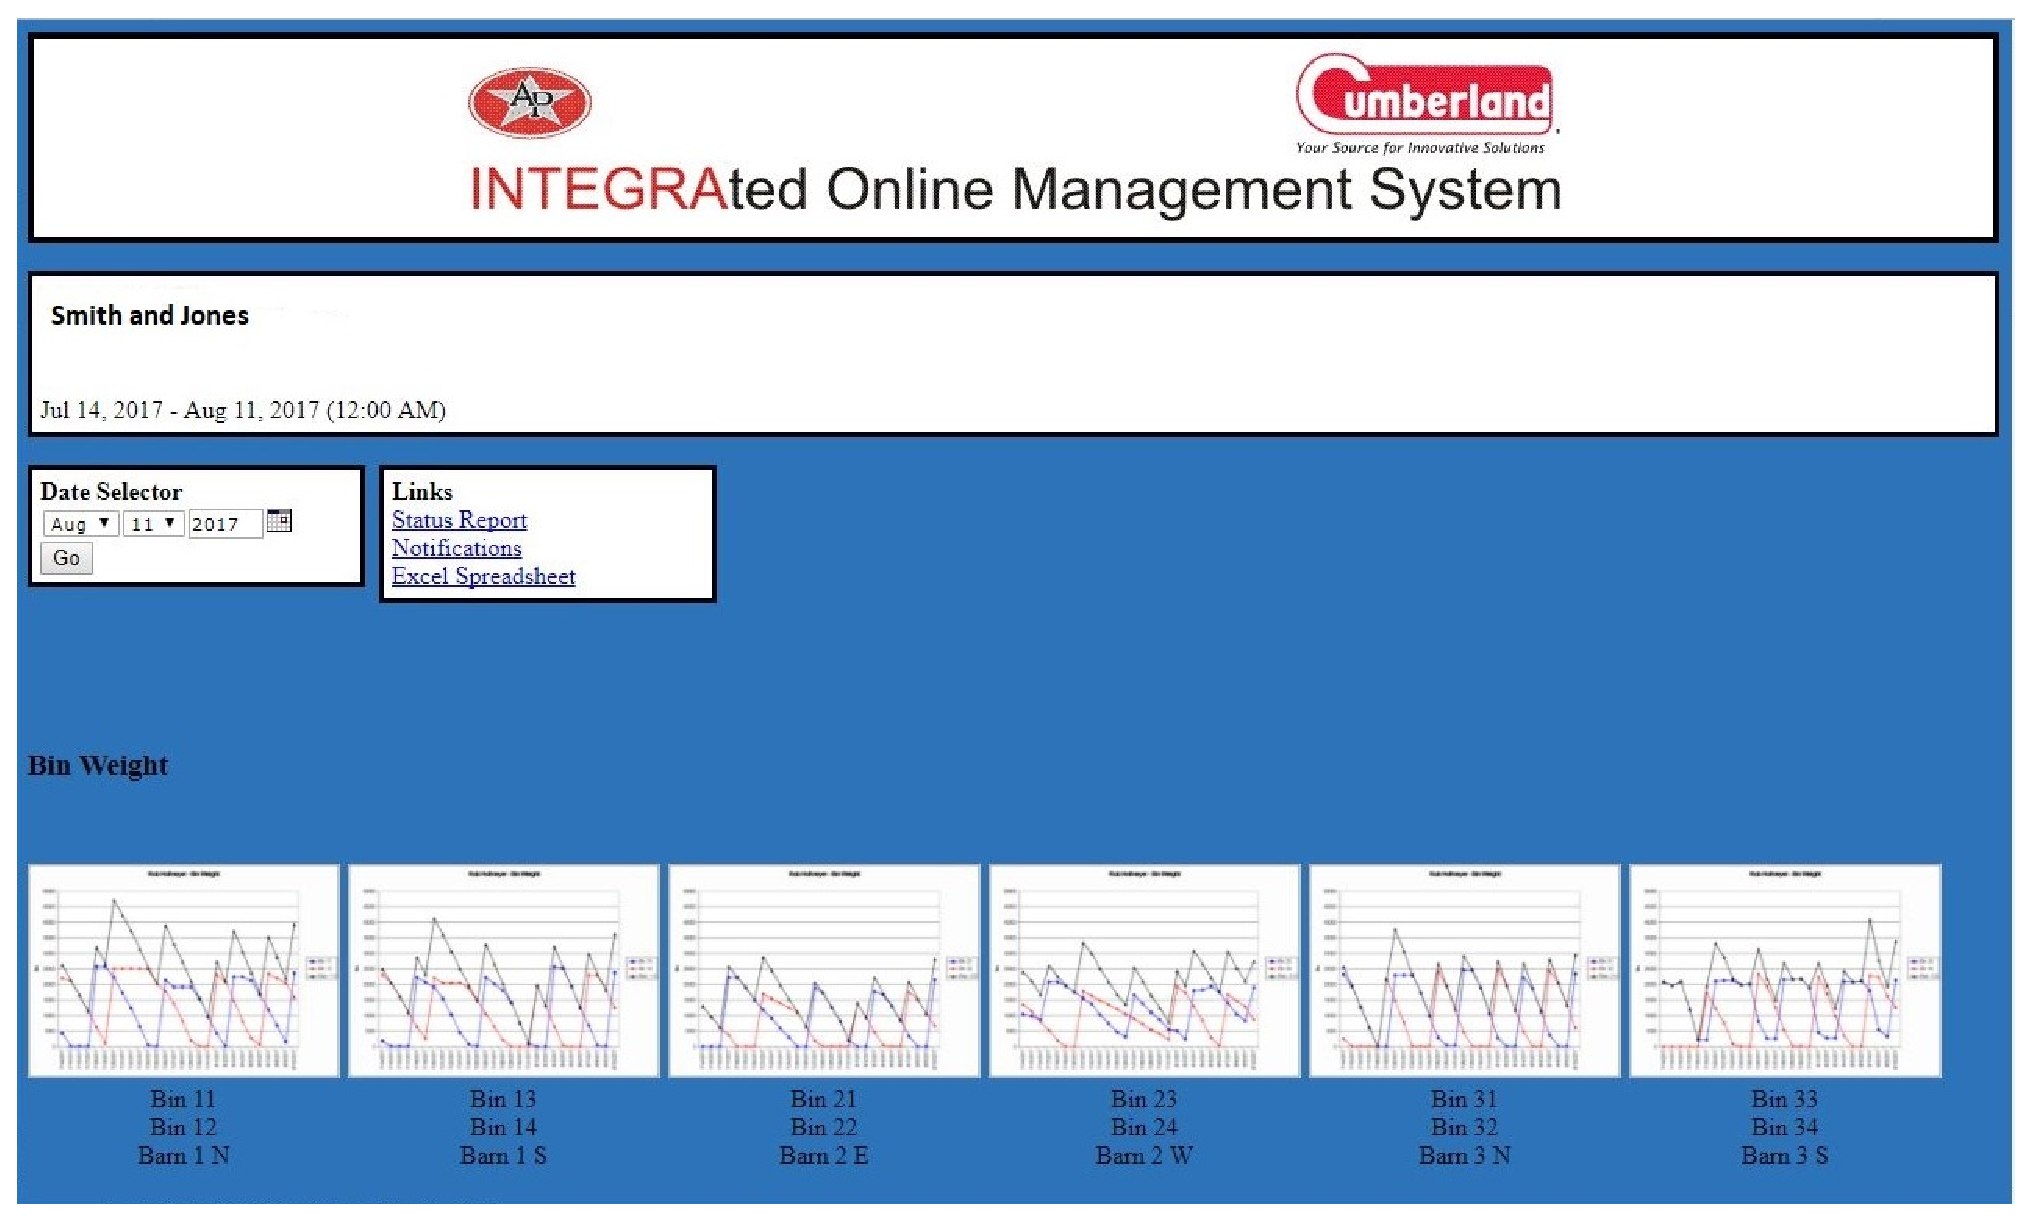
\includegraphics[width=0.9\columnwidth]{dashboard}
    \caption{Dashboard display of Feed-Link system.}
    \label{console}
\end{figure}

Figure~\ref{graph} illustrates data logs collected over a month,
showing the clear correlation between low feed consumption and
high temperatures on two occasions.
This is an indication of the kinds of things that can be
learned from data collected for a single barn.

\begin{figure}[t]
 \centering
\begin{tabular}{c c}
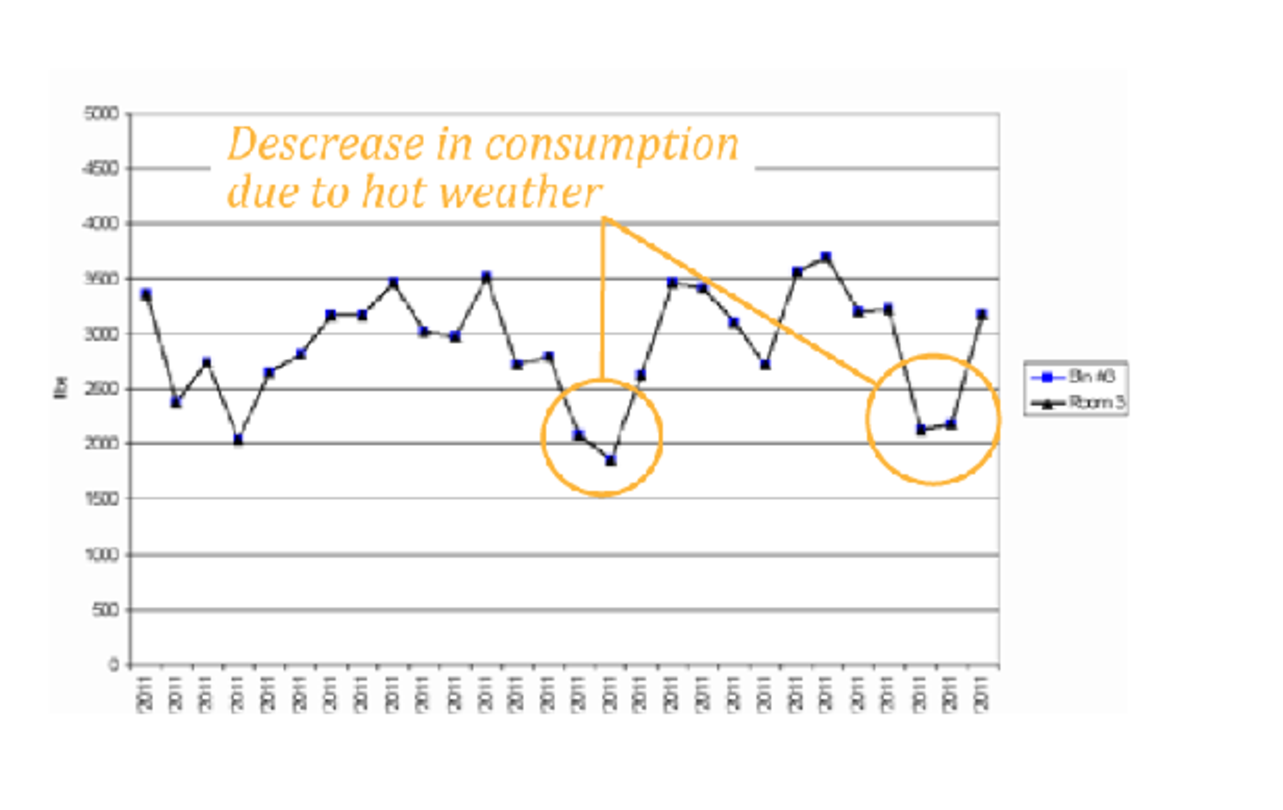
\includegraphics[width=0.45\columnwidth]{hotweather-feed-consumption-600x373} &
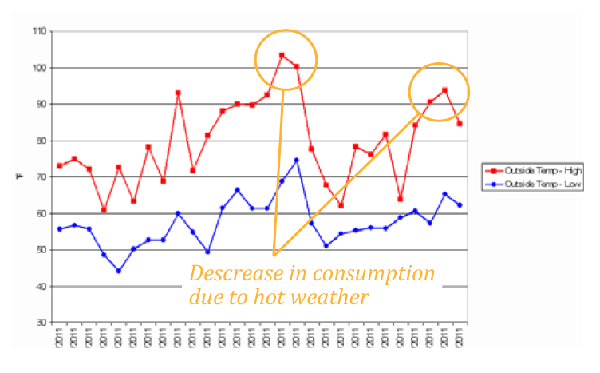
\includegraphics[width=0.45\columnwidth]{hotweather-daily-hi-lo-600x373} \\
(a) Daily feed consumption. & (b) Daily high and low barn temperature.
\end{tabular}
    \caption{Plot of data logs.}
    \label{graph}
\end{figure}

While the two figures show images from a desktop PC screen, modern
remote communications capability is also supported via apps that
run on smartphones and tablets.

In addition to diagnosing the root causes of issues in the barn
the historical logs also enable the tracking of
parameter changes by operators as well as support the demonstration
and documentation of regulatory compliance.
Using Feed-Link, these data logs
are collected automatically and the information retained in the
cloud for easy access by the owners/operators of the equipment (the
farmer, in most instances).

It should be clear that preserving privacy without concurrently
ensuring security would be a completely unacceptable state of affairs.
The security of our systems is
state-of-the-art~\cite{ccgss16,ccgss17b}, with special attention given
to ease-of-use considerations, as there is ample evidence that
security measures that are difficult to implement are frequently
circumvented by users~\cite{gefen2000relative,hertzum2004usable,schneier16}.

Currently, the data access model is such that farmers have
access to data from their own equipment, but there is no data sharing.
Because individual farms each typically have a limited number of
barns (between 1 and 4 would be typical at an
individual facility), there is limited data available for 
learning to take place.  This is true whether the learning is
happening in an automated way (e.g., using modern
machine learning techniques) or manually (using visualization tools).
Each of these approaches will benefit from broader experiential coverage.
Changing this current state of affairs is the specific purpose of this
proposed research project.

\subsection{Privacy Theory}

Our goal is to make aggregated data available while preserving the
privacy of individual data owners (farmers).  Differential privacy
provides strong theoretical guarantees in this area.  Dwork and
Roth~\cite{dwork11,dr14} provided the seminal initial work in this
area, and more recently Nguyen et al.~\cite{nkk13} and
Wang et al.~\cite{wll15} have reviewed the differential
privacy literature as it has been applied to various practical circumstances.
A number of groups have contributed to differentially private hierarchical data
(referred to as histograms)~\cite{hrms10,xxy10}.
Most relevant to our interest is the work of
Rastogi and Nath~\cite{rn10} and
Fan and Xiong~\cite{fx12,fx14}, who describe approaches to time series data.

Differential privacy is far from the only way to tackle the problem.
Others have described approaches such as
$k$-anonymity~\cite{samarati01,sweeney02},
$l$-diversity~\cite{mkgv07},
other techniques aimed at hierarchical data sets~\cite{lnpr14}, and some
have asserted that multiple, combined approaches are superior to any
individual technique~\cite{ct13}.
TIPPERS~\cite{tippers} is an experimental infrastructure, built on a
Honeywell building management system, that supports privacy research
in the IoT space.

The core notion of differential privacy, informally stated, is that whether
or not a single individual chooses to share his/her data to be a part of
the collected data set does not impact the conclusions one draws from
the data set.
This is typically accomplished by perturbing the results of queries
against the data set by some random amount.
Moving towards more formality~\cite{dr14}, a randomized algorithm $\mathcal{M}$
is $(\epsilon,\delta)$-\emph{differentially private} if for all
$\mathcal{S} \subseteq \mbox{Range}(\mathcal{M})$ and datasets $x$ and $y$
differing in at most one record:
\begin{equation}
\Pr[\mathcal{M}(x) \in \mathcal{S}] \leq e^\epsilon \cdot \Pr[\mathcal{M}(y)
\in \mathcal{S}] + \delta
\label{eqn:dp}
\end{equation}
where the probability is over the randomness of the algorithm $\mathcal{M}$.
The parameter $\epsilon$ is often called the
\emph{privacy budget}~\cite{McSherry09}; $(\epsilon,\delta)$-differential
privacy ensures that for all adjacent $x$ and $y$, the privacy loss
(as defined in~\cite{dr14}) will
be bounded by $\epsilon$ with probability at least $1-\delta$.
Operationally, it is possible to achieve differential privacy by adding
i.i.d.~noise to query results.

Our circumstance is one in which time series data is to be queried, and we
wish to preserve the privacy of the data owners (rather than that of
an individual record).
Fan and Xiong~\cite{fx12,fx14} describe a mechanism in which the time
series are first sampled, perturbed (by adding i.i.d.~noise), and then
the released series is composed using prediction (for the non-sampled
points) and prediction-correction (for the sampled points).  It is this
approach that we will initially explore.

